\documentclass[uplatex, a4paper, 12pt, openany, oneside]{jsbook}

\usepackage[dvipdfmx]{graphicx}
\usepackage[dvipdfmx]{color}
\usepackage[dvipdfmx, bookmarks=true, setpagesize=false]{hyperref}
\usepackage{pxjahyper}

\usepackage{thesis}
\usepackage{here}
\usepackage{url}
\usepackage{subcaption}


\thesis{卒 業 論 文}
\title{
  \centering
    \scalebox{1.0}{視覚と行動のend-to-end学習により経路追従行動を}\\
    \scalebox{1.0}{オンラインで模倣する手法の提案}\\
    \scalebox{1.0}{(オフラインでデータセットを収集して訓練する手法の検証)}
    \vspace{-0.3zh}
    \scalebox{0.7}{A proposal for an online imitation method of path-tracking}
    \scalebox{0.7}{behavior by end-to-end learning of vision and action}
    \scalebox{0.7}{(Validation of a method to collect and train datasets offline)}
    \vspace{-5.0zh}
}
\setlength{\textwidth}{\fullwidth}
\setlength{\evensidemargin}{\oddsidemargin}

\date{\today}
\vspace{-15.0zh}
\teacher{林原 靖男 教授}
\vspace{-15.0zh}
\organization{千葉工業大学 先進工学部 未来ロボティクス学科}
\author{19C1068 髙橋祐樹}
\vspace{-15zh}

\renewcommand{\baselinestretch}{1.2}
\begin{document}

%% Front Matter
\frontmatter{}
%
\chapter{結言}
\label{chap:conclusion}
%
%\input{introduction/preface}
%
%!TEX root = ../thesis.tex

本研究では, 経路追従行動をカメラ画像を入力としたend-to-end学習で模倣する岡田ら\cite{okada-si}と清岡ら\cite{kiyooka-si}の手法を基に, 新たなデータセットの収集方法と収集したデータ量を増やすことで, 経路追従行動を獲得できる手法を提案した. 
%
%
%% Main Matter
\mainmatter{}
%
\chapter{結言}
\label{chap:conclusion}
%
%\input{introduction/preface}
%
%!TEX root = ../thesis.tex

本研究では, 経路追従行動をカメラ画像を入力としたend-to-end学習で模倣する岡田ら\cite{okada-si}と清岡ら\cite{kiyooka-si}の手法を基に, 新たなデータセットの収集方法と収集したデータ量を増やすことで, 経路追従行動を獲得できる手法を提案した. 
%
%
\chapter{要素技術}
\label{chap:technology}
%
%\input{introduction/preface}
%
%!TEX root = ../thesis.tex

\section{ディープラーニング}
ディープラーニングとは, 人間の神経細胞を模したネットワーク構造のことである. 主に, 入力層と出力層, その間に中間層(隠れ層)という構成である. 中間層を多層化することで, 複雑な入力情報を処理し, パターンを認識することや, ルールを読み解くことができる. 近年では, 画像や物体認識, 自然言語処理などで活用されている. \figref{Fig:dl}に構造の一例を示す. 

\vspace{30mm}

\begin{figure}[h]
     \centering
     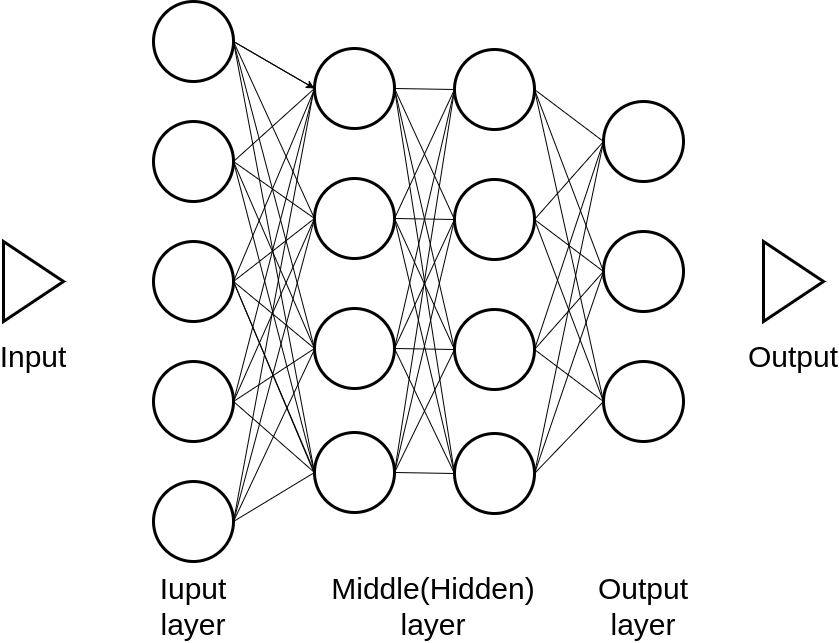
\includegraphics[keepaspectratio, scale=0.3]
     {images/dl.png}
     \caption{Structure of deep learning}
     \label{Fig:dl}
     \end{figure}

\newpage
\section{end-to-end学習}
end-to-end学習とは, 入力から出力までの流れを一括に学習することができる手法である. 例として, 画像中からの文字認識を行う処理を挙げる. 一般的な処理では, \figref{Fig:example}のように画像から文字検出を行い, その後に文字分割, 最終的に文字認識をする. しかし, end-to-end学習では, \figref{Fig:end-to-end}に示すような入力から出力までの流れを一括して学習することができる. 

\vspace{35mm}

\begin{figure}[h]
     \centering
     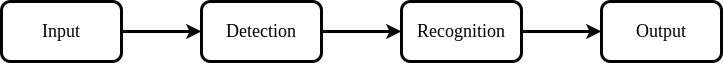
\includegraphics[keepaspectratio, scale=0.5]
     {images/example.png}
     \caption{Structure of general learning}
     \label{Fig:example}
     \end{figure}

\begin{figure}[h]
     \centering
     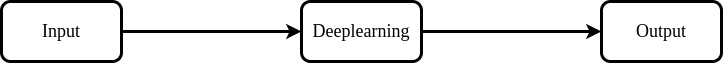
\includegraphics[keepaspectratio, scale=0.5]
     {images/end-to-end.png}
     \caption{Structure of end-to-end learning}
     \label{Fig:end-to-end}
     \end{figure}

\newpage
\section{データセット}
データセットとは, 学習に使用する学習(訓練)データの集合のことである. 例として, \figref{Fig:mnist}に示すような0から9の手書きで書かれた数字の画像セットであるMNISTが挙げられる. 機械学習や画像認識において多く利用されており, 訓練画像6000枚とテスト画像1000枚で構成されている. 

\vspace{5mm}

\begin{figure}[h]
     \centering
     
\includegraphics[keepaspectratio, scale=0.5]
     {images/mnist.png}
     \caption{MNIST dataset(source: \cite{mnist})}
     \label{Fig:mnist}
     \end{figure}

\section{オフライン学習}
オフライン学習とは, あらかじめ用意したデータセットを使用して学習を行うことである. これに対して, 先行研究用で用いたオンライン学習とは, タスクを行いながらデータ収集をし, そのデータを使用して学習することを指す. 

% \section{ミニバッチ学習}
% ミニバッチ学習とは, 訓練データをいくつかのグループ(バッチ)に分けて順番に学習を行うことである. 特徴としては, 勾配更新の頻度が高く, 計算量が少なくて済むといったことが挙げられる. これらの特徴を踏まえて, 先行研究ではオンラインで学習を行うことから, ミニバッチ学習を使用している.
\section{バッチ学習}
バッチ学習とは, 訓練データを一括で処理する学習方法である. 特徴として, 一度に大量のデータを扱うことができるため学習の進行が安定しやすく, 訓練データに異常データが混じっていても受ける影響が小さくて済むなどが挙げられる. また, バッチ学習ではバッチサイズがデータ数となることが多い. 

\section{地図を用いたルールベース制御器によるナビゲーション}
地図を用いたルールベース制御器によるナビゲーションについて説明する. このナビゲーションには, ROSのパッケージであるnavigation\cite{navigation}を使用している. 移動ロボットは, LiDARやホイールオドメトリなどのセンサデータを使用して作成した占有格子地図を用いて目的地まで移動する. そして, 移動ロボットは\figref{Fig:navigation}のように, LiDARやホイールオドメトリなどのセンサデータを入力として, 自己位置推定と経路計画を行い, それらに基づいて自律移動をする. 自己位置推定にはパーティクルフィルタを用いたモンテカルロ自己位置推定(MCL)\cite{mcl1}\cite{mcl2}, 経路計画とモータ指令にはmove\_base\cite{navigation}を使用している.  経路計画では, 動的計画法によって壁や障害物を回避するように経路を生成する. モータ指令は, 生成された経路に従って速度制御を行っている.

% 地図を用いたルールベース制御器によるナビゲーションについて説明する. このナビゲーションには, ROSのパッケージであるnavigation\cite{navigation}を使用している. 移動ロボットは, \figref{Fig:navigation}のようにLiDARのスキャンデータやオドメトリを入力として自己位置推定と経路計画を行い, これらに基づいて自律走行をする. また, 自己位置推定には, amcl(Adaptive Monte Carlo Localization), 経路計画とモータ指令にはmove\_base\cite{navigation}を使用している. 

\begin{figure}[h]
     \centering
     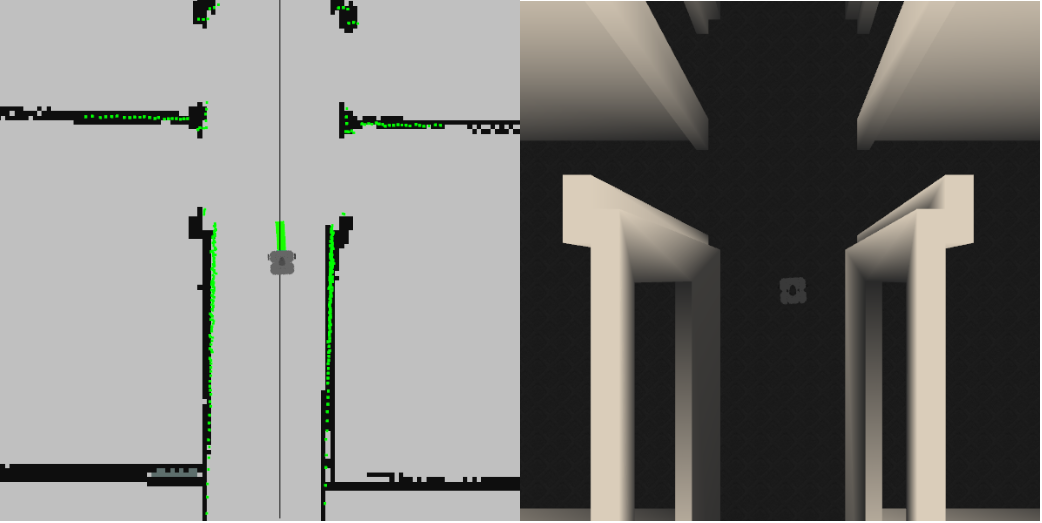
\includegraphics[keepaspectratio, scale=0.3]
     {images/navigation.png}
     \caption{Map based navigation using navigation package}
     \label{Fig:navigation}
     \end{figure}
%
%
\chapter{提案手法(オフライン手法)}
\label{chap:proposed-method}
%
%\input{introduction/preface}
%
%!TEX root = ../thesis.tex

本章では, 従来研究を基にしたオフラインでデータを収集し訓練する手法を提案する.

\section{手法}
本研究で検証するオフライン手法に関して述べる. オンライン手法と比べて, オフライン手法は画像と目標角速度のデータを事前に収集して, 学習するところが異なる. \figref{Fig:collect-data2}にシミュレータを用いて収集するデータを示す. 目標経路(赤線)から一定距離の位置にロボットを配置して, さらに目標経路の方向を基準として, ヨー方向に一定量回転する. その時の中央のカメラの画像と, 目標角速度を収集してデータセットに加える. ちなみに, 本手法でデータを収集するためには, 非常に多くのロボットの置き直しをしなければならない. これを, 実ロボットに応用する際には, 1台のロボットに複数のカメラを搭載して, 経路から一定距離離れた画像を収集する. そうすることで, 置き直ししなくても経路を走行すればデータを集められる. そのため,実ロボットへの応用も可能であると考える. このように収集したデータセットを用いてオフラインで学習する. なお,リアルタイム性に配慮して, オンライン手法ではバッチサイズ8のミニバッチ学習を行っていたが, オフライン学習ではリアルタイム性は必要ないため, バッチ学習を行う. 

% \vspace{10mm}
\newpage
  \begin{figure}[h]
  \centering
  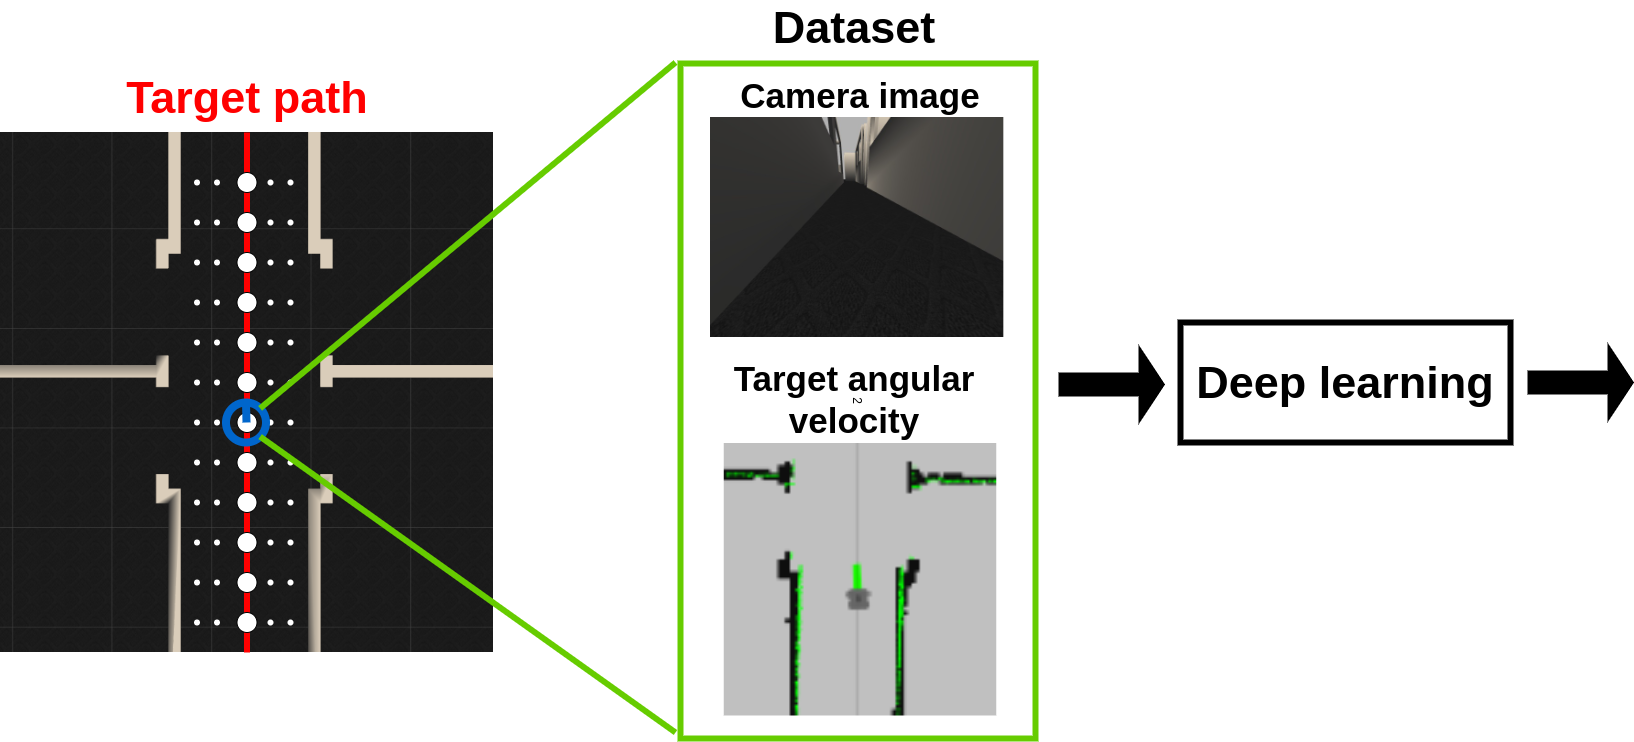
\includegraphics[keepaspectratio, scale=0.2]{images/collect-data2.png}
  \caption{Data collected by the simulator in the learning phase}
  \label{Fig:collect-data2}
  \end{figure}


%
%
\chapter{結言}
\label{chap:conclusion}
%
%\input{introduction/preface}
%
%!TEX root = ../thesis.tex

本研究では, 経路追従行動をカメラ画像を入力としたend-to-end学習で模倣する岡田ら\cite{okada-si}と清岡ら\cite{kiyooka-si}の手法を基に, 新たなデータセットの収集方法と収集したデータ量を増やすことで, 経路追従行動を獲得できる手法を提案した. 
%
%% Back Matter
\backmatter{}
%
%!TEX root = ../thesis.tex
%\bibliographystyle{plain}
\bibliographystyle{junsrt}
%\bibliography{report}
\nocite{*}
% \bibliography{main_bibliography}
%!TEX root = ../thesis.tex
% \chapter*{参考文献}
\addcontentsline{toc}{chapter}{参考文献}

\begin{thebibliography}{99}

  \bibitem{okada-si2020}
  岡田 眞也, 清岡 優祐, 上田 隆一, 林原 靖男: ``視覚と行動のend-to-end学習により経路追従行動をオンラインで模倣する手法の提案'', \textit{計測自動制御学会 SI 部門講演会 SICE-SI2020 予稿集}, pp.1147-1152, 2020.

  \bibitem{okada-si2021}
  岡田 眞也, 清岡 優祐, 春山 健太, 上田 隆一, 林原 靖男: ``視覚と行動のend-to-end学習により経路追従行動をオンラインで模倣する手法の提案 -経路追従行動の修正のためにデータセットを動的に追加する手法の検討'', \textit{計測自動制御学会 SI 部門講演会 SICE-SI2021 予稿集}, pp.1066-1070, 2021.

  \bibitem{bojaski}
  Mariusz Bojarski et al., ``End to End Learning for Self-Driving Cars.'', arXiv: 1604.07316(2016). 

  \bibitem{Jing}
  Jing Bi, Tianyou Xiao, Qiuyue Sun, Chenliang Xu., ``Navigation by Imitation in a Pedestrian-Rich Environment,'' arXiv preprint arXiv:1811.00560, 2018.

  \bibitem{navigation}
  ros-planning, navigation
  \url{https://github.com/ros-planning/navigation}
  (最終閲覧日: \today)

  \bibitem{mcl1}
  F. Dellaert, Fox D., Burgard W., and S Thrun. “Monte carlo localization for mobile robots“. Proceedings 1999 IEEE international conference on robotics and automation (Cat. No. 99CH36288C), Vol. 2, pp. 1322–1328, 1999.

  \bibitem{mcl2}
  D. Fox, W. Burgard, F. Dellaert, and S. Thrun. “ Monte carlo localization: Efficient position estimation for mobile robots“. AAAI/IAAI, Vol. 2-2, pp. 343–349, 1999.

  \bibitem{mnist}
  The MNIST database of handwritten digits
  \url{http://yann.lecun.com/exdb/mnist/}
  (最終閲覧日: \today)

  \bibitem{offline}
  髙橋 祐樹, 白須 和暉, 藤原 柾, 上田 隆一, 林原 靖男: ``視覚と行動のend-to-end学習による経路追従行動の模倣 -データセットを収集してオフラインで訓練する手法の検討-'', 日本機械学会ロボティクス・メカトロニクス講演会2023講演論文集, 2P1-G07, 2023.

  \bibitem{gazebo}
  gazebo.
  \url{http://gazebosim.org/.}
  (最終閲覧日: \today)

  \bibitem{willow}
  Koenig and Nathan and Andrew Howard., ``Design and use paradigms for gazebo, an open-source multi-robot simulator.'' 2004 IEEE/RSJ International Conference on Intelligent Robots and Systems (IROS)(IEEE Cat. No. 04CH37566). Vol. 3. IEEE, pp.2149-2154(2004).
  (最終閲覧日: \today)

  \bibitem{turtlebot3}
  Turtlebot3 — robotis emanual.robotis.
  \url{https://emanual.robotis.com/docs/}
  (最終閲覧日: \today)

\end{thebibliography}
% \input{main_bibliography}
%
%!TEX root = ../thesis.tex
\chapter*{付録}
\addcontentsline{toc}{chapter}{付録}
成功や失敗した際のロボットの走行の軌跡を掲載(一例)

%
%!TEX root = ../thesis.tex
\chapter*{謝辞}
\addcontentsline{toc}{chapter}{謝辞}

本研究を進めるにあたり,1年に渡り, 熱心にご指導を頂いた林原靖男教授に深く感謝いたします.また, 日頃から研究へのアドバイス, 指導, サポートしてくださった清岡優祐様, 春山健太様, 藤原柾様, 白須和暉様, 並びにロボット設計制御研究室の皆様には, 心から深く感謝を申し上げます. 
%


%

\end{document}
